\documentclass[12pt, a4paper, titlepage, table]{article}
\usepackage{pdfpages}
\usepackage[utf8]{inputenc}
\usepackage[T1]{fontenc}
\usepackage{titlesec}
\usepackage[french]{babel}
\usepackage{caption}
\usepackage{float}
\usepackage{graphicx}
\usepackage[inner=2cm, outer=2cm, top=2cm, bottom=2cm]{geometry}
\usepackage[T1]{fontenc}
\usepackage{times}
\usepackage{xr} 
\usepackage{multirow}
\usepackage{amsmath}
\usepackage{array}
\usepackage{booktabs}

\begin{document}
	\label{document}
	\title{Etude d'un MOOC}
	\author{Sébastien Mertès}
	\date{\today}
	\maketitle
	\renewcommand{\thesection}{\arabic{section}.}
	\renewcommand{\thesubsection}{\thesection\arabic{subsection}}
	\renewcommand{\tablename}{Tableau}
	\renewcommand{\abstractname}{Résumé}
	\captionsetup[table]{font={small}}
	\setlength{\parindent}{0pt}
	\captionsetup{labelfont=bf}
	\tableofcontents

\newpage	
\section{Principales variables utilisées}
Les principales variables utilisées dans cette analyse sont listées dans le Tableau 1. Il s'agit d'un jeu de données résultant d'une base d'apprenants à un MOOC et d'une autre base indiquant leurs parcours d'apprentissage par le suivi ou non des vidéos et le passage des quiz, de l'examen ou de la certification du MOOC. La formation du MOOC s'étend sur 5 semaines. L'indication des vidéos consultées est donnée par les variables S1 à S5 correspondant au numéro de la semaine  ainsi qu'aux quiz.
Le passage ou non de la certification et de l'examen est donné par les variables Exam.bin et Certif.bin. Le genre de l'apprenant est donnée par la variable Gender ainsi que son HDI par la variable Country\_HDI.

\begin{table}[H]
	\centering
	\fontsize{10}{12}\selectfont
	\begin{tabular}{|r|r|}
	\hline 
	\multicolumn{1}{|c|}{\textbf{Variable}}& 
	\multicolumn{1}{c|}{\textbf{Type}} \\
	\hline
   	Student\_ID&             int64\\      
   	Gender    &             object\\
	Country\_HDI&            object\\
	Exam.bin    &           bool\\   
	Assignment.bin&         int64\\  
	Quizz.1.bin&            int64 \\ 
	Quizz.2.bin&            int64 \\ 
	Quizz.3.bin&            int64 \\
	Quizz.4.bin&            int64 \\ 
	Quizz.5.bin&            int64 \\ 
	S1.L1      &            int64 \\ 
	S1.L2      &            int64 \\ 
	S1.L3      &            int64 \\ 
	S1.L4      &            int64 \\ 
	S1.L5      &            int64 \\
	S1.L6      &            int64 \\ 
	S2.L1      &            int64 \\ 
	S2.L2      &            int64 \\ 
	S2.L3      &            int64 \\ 
	S2.L4      &            int64 \\ 
	S2.L5      &            int64 \\ 
	S2.L6      &            int64 \\  
	S3.L1.1    &            int64 \\ 
	S3.L1.2    &            int64 \\ 
	S3.L2      &            int64 \\ 
	S3.L3      &            int64 \\ 
	S3.L4      &            int64 \\ 
	S3.L5      &            int64 \\ 
	S4.L1.1    &            int64 \\ 
	S4.L1.2    &            int64 \\ 
	S4.L2      &            int64 \\ 
	S4.L3      &            int64 \\ 
	S4.L4      &            int64 \\ 
	S4.L5      &           	int64 \\   
	S5.L1.1    &            int64 \\ 
	S5.L1.2    &            int64 \\ 
	S5.L2      &            int64 \\ 
	S5.L3      &            int64 \\ 
	S5.L4      &            int64 \\ 
	S5.L5      &            int64 \\ 
	Certif.bin &           bool  \\
	\hline
	\end{tabular}
	\caption{\textbf{Proportions des apprenants par type et par itération.}}
\end{table}  

\newpage
\section{Proportions des types d'apprenants par itération}
Le Tableau 2 montre la proportion de chacun des types d'apprenant par itération,  auditing, bystander, completer et disengaging par itération. Cela en fonction du nombre de vidéos vues, de quiz réalisés et du passage de l'examen ou de la certification ou non.

\begin{table}[H]
	\centering
	\fontsize{10}{12}\selectfont
	\begin{tabular}{|c|l|r|r|r|}
		\hline 
		\multicolumn{1}{|c|}{\textbf{Itération}} & 
		\multicolumn{1}{c|}{\textbf{Type}} &
		\multicolumn{1}{c|}{\textbf{Total/type}}&
		\multicolumn{1}{c|}{\textbf{Total/itération}}&
		\multicolumn{1}{c|}{\textbf{Pct/Type}}\\
		\hline
		1&	Auditing&		1207&	7965&	15.2\%\\
		1&	Bystander&		4285&	7965&	53.8\%\\
		1&	Completer&		20	&	7965&	0.3\%\\
		1&	Disengaging&	2453&	7965&	30.8\%\\
		2&	Auditing&		538	&	3702&	14.5\%\\
		2&	Bystander&		2168&	3702&	58.6\%\\
		2&	Completer&		876	&	3702&	23.7\%\\
		2&	Disengaging&	120	&	3702&	3.2\%\\
		3&	Auditing&		375	&	3515&	10.7\%\\
		3&	Bystander&		2238&	3515&	63.7\%\\
		3&	Completer&		832	&	3515&	23.7\%\\
		3&	Disengaging&	70	&	3515&	2.0\%\\
		\hline
	\end{tabular}
\caption{\textbf{Proportions des apprenants par type et par itération.}}
\end{table}

\section{Test d'indépendance du $\chi2$ entre le genre et l'HDI}

La Figure 1 représente les résidus du test d'indépendance fondé sur le chi2 entre le genre et l'HDI, afin de déterminer si il y un lien entre l'Human 
Development Index et le genre (homme ou femme).
Les cellules rouges indiquent que le modèle prédit (calculé) a sous-évalué la valeur observée puisque le résidu est positif. Et réciproquement, 
la couleur bleu indique un résidu négatif, indiquant que le modèle prédiction a sur-évalué la valeur observée. 

Nous remarquons que les personnes venant des pays très développés (TH) sont surrepresentées et les hommes seraient 2 fois plus nombreux dans cette étude. 

Le Tableau 3 indique le tableau de contingence des fréquences observées entre les variables catégorielles genre et HDI. 
Chacune comprenant respectivement 2 et 3 modalités. C'est à partir des valeurs de ce tableau que nous pouvons appliquer le test du $\chi^2$ et en déduire 
si les variables sont statistiquement indépendantes ou non en appliquant le formule du V de Cramer.

\begin{table}[H]
	\centering
	\fontsize{10}{12}\selectfont
	\begin{tabular}{|c|l|r|r|r|}
		\hline 
		\multicolumn{1}{|c|}{\textbf{}} & 
		\multicolumn{1}{c|}{\textbf{B}} &
		\multicolumn{1}{c|}{\textbf{I}} &
		\multicolumn{1}{c|}{\textbf{TH}} \\
		\hline
 			Femme&	147&	233&	2545\\
 			Homme&	883&	432&	4711\\
		\hline
	\end{tabular}
\captionof{table}{\textbf{Tableau de contingence du genre et de l'HDI.}}
\end{table}

	\begin{figure}[H]
		\centering
		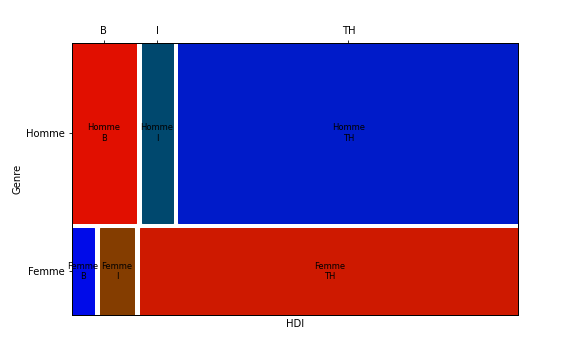
\includegraphics[width=1\textwidth]{../../graph/mosaic_contingence.png}
		\captionof{figure}{\textbf{Mosaic des résidus du test du $\chi2$}}
	\end{figure}

La Figure 2, représente les résidus du modèle observé par rapport au modèle de prédiction. Nous observons que les écarts des résidus sont assez éloignés 
de la droite droite horizontale faisant référence à des écarts nuls entre les valeurs observées et calculées. Nous pouvons observer que le modèle de 
prédiction est assez éloigné des observations.

	\begin{figure}[H]
		\centering
		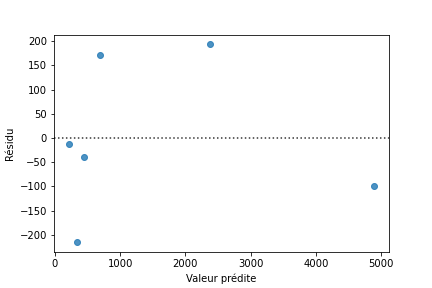
\includegraphics[width=0.7\textwidth]{../../graph/residus_chi2.png}
		\captionof{figure}{\textbf{Résidus du test du $\chi2$}}
	\end{figure}


La formule de Cramer ci-dessous, mesure la force de l'association entre deux variables catégorielles.
\[ V = \sqrt{\frac{\chi^2}{n \cdot (\min(r, c) - 1)}} \]
V représente le coefficient de Cramer,  r est le nombre de modalités de la première variable et c'est le nombre de modalités de la deuxième variable.
Nous allons appliquer cette formule aux variables précédentes indiquant le genre et HDI.
L'index HDI a 3 modalités (c) et le genre a 2 modalités (r), la valeur V est de 0,14.
Le tableau 4, résume les valeurs statistiques du test du $\chi^2$ et du V de Cramer.

\begin{table}[H]
	\centering
	\fontsize{12}{20}\selectfont
	\begin{tabular}{|l|r|}
		\hline  
		$\chi2$&	179.24\\
		p-value&	1.17\\
		V-Cramer&	0.14\\
		\hline
	\end{tabular}
	\caption{\textbf{Valeurs du $\chi2$ et du V de Cramer.}}
\end{table}

L'hypothèse de départ sur l'indépendance du genre et de l'HDI serait confirmé puisque la dépendance de ces catégories est statistiquement non significatif 
(p-value > 11 \%) et la valeur du V de Cramer est très faible (proche de 0). Nous pouvons donc envisager qu'il n'y a pas de lien entre le genre et l'index HDI.

\section{Modèle linéaire, tests non paramétriques}
\subsection{Tests statistiques entre le nombre de vidéos visionnées et le genre}

Après l'index HDI, intéressons-nous aux nombres de vidéos vues par rapport au genre. Le figure 3 montre le nombre moyen de visionnage pour les femmes et 
les hommes. Son observation montrerait qu'en moyenne il y aurait une très faible différence entre les hommes et les femmes sur le nombre de vidéos vues. 

	\begin{figure}[H]
		\centering
		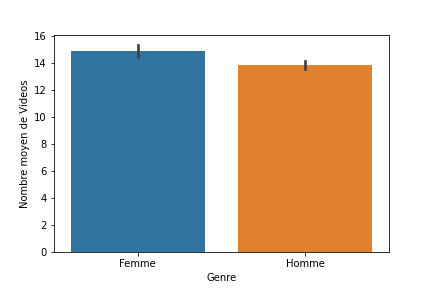
\includegraphics[width=0.7\textwidth]{../../graph/mean_video.png}
		\caption{\textbf{Moyenne des vidéos vues par genre.}}
	\end{figure}

L'hypothèse de départ (H0) est qu'il n'y a aucune différence sur le nombre de vidéos vues entre les hommes et les femmes. La figure 4, montre la distribution du nombre de vidéos vues par genre. Nous pouvons constater que la distribution des données ne ressemble pas à une distribution normale.

	\begin{figure}[H]
		\centering
		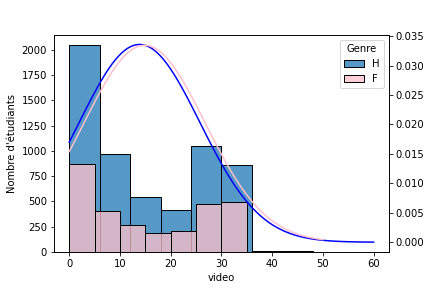
\includegraphics[width=0.8\textwidth]{../../graph/distribution_video.png}
		\caption{\textbf{Distribution du nombre de vidéos visionnées par genre.}}
	\end{figure}

La Figure 5, compare les quantiles de la distribution des vidéos des 2 modalités homme et femme afin de déterminer graphiquement si la distribution est normale. Nous observons également que la distribution observée ne suit pas la distribution théorique normale. Cela confirmerait l'hypothèse que la distribution observée n'est pas gaussienne.


  	\begin{figure}[H]
  		\centering
  		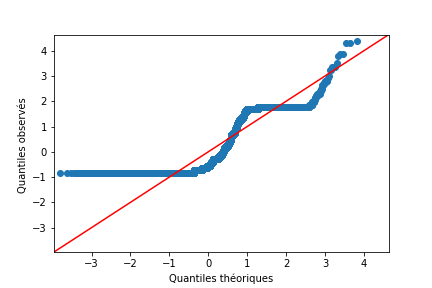
\includegraphics[width=0.8\textwidth]{../../graph/distribution_video3.png}
  		\caption{\textbf{Normalité de la distribution du nombre de vidéo.}}
  	\end{figure}
  
La taille des échantillons étant conséquente nous pouvons appliquer le test de Kolmogrov-Smirnov (KS) pour vérifier la normalité des données. 
L'hypothèse de départ (H0) est que la distribution est gaussienne.
Le résultat de ce test donnant une valeur de 0 de la p-value, la normalité n'est pas statistiquement significative et conclure qu'il est fortement probable 
que celle-ci ne l'est pas.   
En conséquence des différents tests de normalité de la distribution des données du nombre de vidéos pour les 2 modalités homme et femme, il est indiqué
de procéder à un test non paramétrique afin de déterminer si il y a une différence sur le nombre de vidéos visonnées entre hommes et femmes. 

Le Tableau 5 affiche les valeurs du test non paramétrique de Mann-Whitney U. Les résultats des statistiques de test U appliquées au genre, montreraient 
qu'il y a une différence significative (p = 0\%) entre le nombre de vidéos vues entre les hommes et les femmes. 
Il semblerait que les femmes consommeraient bien davantage de vidéos en sachant que les hommes sont surreprésentés dans cette étude. 

\begin{table}[H]
	\centering
	\fontsize{12}{20}\selectfont
	\begin{tabular}{|c|c|}
		\hline
		\multicolumn{2}{|c|}{\textbf{Test Mann-Whitney U}}\\ 
		\hline 
		statistic (homme)& 8200580.5\\
		statistic (femme)& 8994696.5\\
		p-value& 0\%\\
		\hline
	\end{tabular}
\captionof{table}{\textbf{Test non paramétriques.}}
\end{table}

\subsection{Tests statistiques entre le nombre de vidéos visionnées et le nombre de quiz réalisés.}
Afin de déterminer quel test de corrélation à appliquer, il est nécessaire de savoir si les données suivent une distribution normale ou non. 
En l'absence de normalité de distribution du nombre de vidéos, on utilisera un test de Spearman afin de tester la corrélation entre le nombre de vidéos 
visionnées et le nombre de quiz. 
Selon les résultats obtenus dans le Tableau 6 du test de Spearman, il y aurait une forte corrélation (0.8) entre le nombre de vidéos vues et le nombre 
de quiz réalisés par un étudiant. 
La corrélation observée est statistiquement significative (p-value=0).
\begin{table}[H]
	\centering
	\fontsize{12}{20}\selectfont
	\begin{tabular}{|c|c|}
		\hline
		\multicolumn{2}{|c|}{\textbf{Test de Spearman}}\\ 
		\hline 
		statistic& 0.80\\
		p-value& 0\\
		\hline
	\end{tabular}
	\caption{\textbf{Test de corrélation.}}
\end{table}

La Figure 6, représente le scatter plot des valeurs observées et le modèle de régression linéaire par la droite tracée en rouge entre le nombre de quiz
effectués et le nombre de vidéos visionnées. Cependant, le modèle linéaire théorique extrapolerait un nombre de quiz bien supérieur à 10 au delà de 60 vidéos 
visionnées alors que la tendance des valeurs observées suggère un plafonnement du nombre de quiz à 10. 
La fonction linéaire ne serait pas le modèle le plus adapté comparé aux données réelles.

\begin{figure}[H]
	\centering
	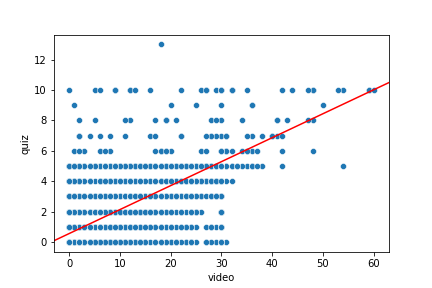
\includegraphics[width=0.8\textwidth]{../../graph/scatter2_regression.png}
	\caption{\textbf{valeurs observées (bleu) et modèle de régression linéaire (rouge).}}
\end{figure}

Le Tableau 7 indique les résultats du modèle de régression linéaire de la variable dépendante quiz et de la variable explicative video. Le $R^2$ à 0.64, 
indiquerait que les valeurs prédites représenteraient 64\% des valeurs observées. 
Selon les résultats du tableau 8, la p-value étant de 0, il y aurait statistiquement un lien sur le nombre de vidéos vues et le nombre de quiz effectués. 
Selon le modèle théorique, il y aurait presque 5 fois moins de quiz effectués que de nombre de vidéos visionnées.

\begin{table}[H]
	\centering
	\fontsize{12}{20}\selectfont
	\begin{tabular}{|ll|ll|}
		\hline
			Dep. Variable:&	quiz&	R-squared:&	0.646\\
			Model:&	OLS&	Adj. R-squared:&	0.646\\
			Method:&	Least Squares&	F-statistic:&	2.653e+04\\
			No. Observations:&	14557&	AIC:&	4.997e+04\\
			Df Residuals:&	14555&	BIC:&	4.998e+04\\
		\hline
	\end{tabular}
\caption{\textbf{Résultats du modèle de régression linéaire (video vs squiz).}}
\end{table}
	
	
\begin{table}[H]
	\centering
	\fontsize{12}{20}\selectfont
	\begin{tabular}{|l|r|r|r|r|}
		\hline
			\multicolumn{1}{|c|}{\textbf{}}&
			\multicolumn{1}{c|}{\textbf{coef}}&
			\multicolumn{1}{c|}{\textbf{std err}}&
			\multicolumn{1}{c|}{\textbf{t}}&
			\multicolumn{1}{c|}{\textbf{p-value}}\\	
		\hline
		\textbf{Réf: Quiz}&	0.5652&	0.014&	39.183&	0***\\
		\textbf{video}&	0.1575&	0.001&	162.896&	0***\\
		\hline
\end{tabular}
\caption{\textbf{Modèle de régression-vidéo vs quiz.}}
\end{table}

	\subsection{ANOVA sans intéraction sur le nombre de vidéos vues selon le genre et l'HDI}
	
	D'après le Tableau 9, le degrés de liberté (df) pour le genre est de 1 car la variable contient 2 modalités (homme et femme).
	En effet, une modalité de la variable est utilisée comme référence dans le modèle.
	\[ df = n[mod] - 1 \]
	Avec n représentant le nombre de modalités (mod) des variables, Genre et New\_HDI.
	La variable Genre comporte 2 modalités (homme et femme) donc le df est de 1. La variable HDI comporte 3 modalités (TH, I, B), 
	donc le df est de 2. Selon le test F de l'ANOVA (F=260), l'indice de développement du pays (HDI) dans lequel les individus vivent aurait
	davantage de lien sur le nombre moyen de vidéos vues que le fait d'être un homme ou une femme (F=11.43).
	  
	\begin{table}[H]
		\centering
		\fontsize{12}{20}\selectfont
		\begin{tabular}{|l|r|r|r|r|r|}
			\hline
					\multicolumn{1}{|c|}{\textbf{}}&
					\multicolumn{1}{c|}{\textbf{df}}&
					\multicolumn{1}{c|}{\textbf{sum\_sq}}&
					\multicolumn{1}{c|}{\textbf{mean\_sq}}&
					\multicolumn{1}{c|}{\textbf{F}}&
					\multicolumn{1}{c|}{\textbf{PR(>F)}}\\
			\hline
				\textbf{Genre}&	1&	1554.89&	1554.9&	11.43&	0***\\
				\textbf{HDI}&	2&	70714.83&	35357.41&	260.08&	0***\\
				\textbf{Residual}&	8861.0&	1204643&	135.95&		&		\\
			\hline
		\end{tabular}
		\caption{\textbf{Table d'ANOVA sans interaction - vidéo vs genre et HDI.}}
	\end{table}

	La sortie du modèle de régression du Tableau 10, décrit la relation statistique entre les variables explicatives, Genre et HDI 
	avec la variable de réponse vidéo. L'équation linéaire résultante du modèle de régression est de la forme : 
	\[ Y=\beta0 + \beta1X1 + \beta2X2 + \beta3X3 \]
	
	Avec :\\
	$Y =$ nombre de vidéos visionnées\\
	$\beta0 = 7.0011$\\
	$\beta1 = 0.0959, X1 = Genre(homme)$\\
	$\beta2 = 4.6774, X2 = HDI(I)$\\
	$\beta3 = 8.6728, X3 = HDI(TH)$\\
	
	Le groupe des femmes et l'index B de l'HDI sont utilisés comme référence dans le modèle.
	En effet, le coefficient $\beta0$ correspond au nombre moyen de vidéos visionnées par les femmes dans la catégorie B. 
	Les catégories TH ($X3$) et I ($X2$), sont comparées à l'index B.
	Ainsi, la différence sur le nombre moyen de vidéos vues est indépendant (p-value de 72 \%) des hommes ($X1$) par rapport aux femmes, contrairement aux apprenants des pays moyennement ou très développés (HDI I et TH) par rapport aux pays pauvres.
	En comparaison des apprenants des pays pauvres (t=8\%), ce serait les apprenants des pays très développés (TH) qui aurait significativement le plus d'influence (t=22\%) sur le nombre moyen de vidéos vues. 
	\begin{table}[H]
		\centering
		\fontsize{12}{20}\selectfont
		\begin{tabular}{|l|r|r|r|r|}
			\hline
			\multicolumn{1}{|c|}{\textbf{}}&
			\multicolumn{1}{c|}{\textbf{coef}}&
			\multicolumn{1}{c|}{\textbf{std err}}&
			\multicolumn{1}{c|}{\textbf{t}}&
			\multicolumn{1}{c|}{\textbf{p-value}}\\	
			\hline
			\textbf{Réf: Genre Femme/HDI B}&			7.0011&		0.432&	16.211&	0***\\	
			\textbf{Genre Homme}&	-0.0959&	0.267&	-0.360&	0.719\\
			\textbf{HDI I}&	4.6774&		0.586&	7.979&	0***\\
			\textbf{HDI TH}&	8.6728&		0.395&	21.937&	0***\\
			\hline
		\end{tabular}
		\caption{{Modèle de régression-vidéo vs genre et HDI (sans interaction).}}
	\end{table}	

	Cependant, le tableau 11 indique un $R^2$ très faible de 5,7\%. Cela indique clairement que le modèle de régression linéaire utilisé n'est pas
	du fidèle aux valeurs observées. 
	\begin{table}[H]
		\centering
		\begin{tabular}{@{}ll@{}}
		\toprule
		Dep. Variable & video \\
		\midrule
		Model         & OLS   \\
		Method        & Least Squares \\
		R-squared     & 0.057 \\
		Adj. R-squared& 0.056 \\
		F-statistic   & 177.2 \\
		\bottomrule
		\end{tabular}
		\caption{Résultats de la régression OLS}
	\end{table}

	\subsection{ANOVA avec interactions sur le nombre de vidéos selon le genre et l'HDI}	
	Dans le Tableau 12, nous testons comment les pays développés (I) ou très développeé (TH ) ont un effet sur le nombre de vidéos visionnées par les hommes par rapport aux femmes et aux pays pauvres (HDI B).   
	Le nombre de vidéos visionnées dépend davantage (t=8.5) et très significativement (p=0\%) des apprenants des pays très développés par rapport aux apprenants des pays pauvres.  
	Cependant, le niveau de développement des pays très développés à significativement un effet (p=4.8\%) sur le nombre de vidéos vues par les hommes par rapport aux femmes.  
	
	\begin{table}[H]
		\centering
		\fontsize{12}{20}\selectfont
		\begin{tabular}{|l|r|r|r|r|}
			\hline
			\multicolumn{1}{|c|}{\textbf{}}&
			\multicolumn{1}{c|}{\textbf{coef}}&
			\multicolumn{1}{c|}{\textbf{std err}}&
			\multicolumn{1}{c|}{\textbf{t}}&
			\multicolumn{1}{c|}{\textbf{p-value}}\\	
			\hline
				\textbf{Réf: Genre Femme/HDI B}&			7.3310&			0.968&	7.573&	0***\\
				\textbf{Genre Homme}&	-0.4810&		1.046&	-0.460&	0.646\\	
				\textbf{HDI I}&	2.7733&			1.236&	2.244&	0.025*\\	
				\textbf{HDI TH}&	8.4673&			0.995&	8.506&	0***\\	
				\textbf{Genre Homme:HDI I}&	2.8032&	1.415&	1.982&	0.048*\\
				\textbf{Genre Homme:HDI TH}&	0.1933&	1.085&	0.178&	0.859\\
			\hline
		\end{tabular}
	\caption{\textbf{Modèle de régression-vidéo vs genre et HDI (avec interaction).}}
\end{table}
	
	D'après le Tableau 13, nous observons que le niveau de développement d'un pays (HDI) a significativement (p-value=0\%) bien davantage d'influence (F=260) sur le nombre moyen de vidéos 
	visionnées quelque soit le sexe. Nous remarquons également, que le nombre de vidéos vues varie statistiquement (p=3\%) faiblement (t=3.5) en fonction  
	du niveau de développement du pays dans lequel les hommes et les femmes vivent. Mais le genre n'a significativement (p = 0) que très faiblement (F=11,44) un impact sur le nombre de vidéos visionnées.
	
	\begin{table}[H]
		\centering
		\fontsize{12}{20}\selectfont
		\begin{tabular}{|l|r|r|r|r|r|}
			\hline
			\multicolumn{1}{|c|}{\textbf{}}&
			\multicolumn{1}{c|}{\textbf{df}}&
			\multicolumn{1}{c|}{\textbf{sum\_sq}}&
			\multicolumn{1}{c|}{\textbf{mean\_sq}}&
			\multicolumn{1}{c|}{\textbf{F}}&
			\multicolumn{1}{c|}{\textbf{PR(>F)}}\\
			\hline
				\textbf{Genre}&	1&	1554.89&	1554.89&	11.44&	0***\\
				\textbf{HDI}&	2&	70714.83&	35357.41&	260.22&	0***\\
				\textbf{Genre:HDI}&2&	954.15&	477.076535&	3.511225&0.03*\\
				\textbf{Residual}&	8859&	1203688&	135.87&	&	\\
			\hline
		\end{tabular}
	\caption{\textbf{Table d'ANOVA avec interaction - video vs genre et HDI.}}
\end{table}


\section{Régression logistique}
\subsection{Régression binomiale}
Nous allons maintenant utiliser une régression binomiale afin de déterminer qui, entre les hommes et les femmes ainsi que des
différents niveaux d'HDI, a davantage de chance de réussite à l'examen ou à la certification dans la version 2 du MOOC.
Le Tableau 14 retranscrit les résultats de cette régression.

	\begin{table}[H]
		\centering
		\begin{tabular}{@{}lllll@{}}
		\toprule
		Description & OR & CI [2.5\% & 97.5\%] & p-value \\
		\midrule
		Réf Gender homme & & & & \\
		Gender femme & 1.021 & 0.851 & 1.224 & 0.826 \\
		Réf HDI B & & & & \\
		HDI TH & 1.558 & 1.149 & 2.113 & 0.004** \\
		HDI I & 1.046 & 0.660 & 1.658 & 0.849 \\
		\bottomrule
		\end{tabular}
		\caption{OR - CI MOOC V2}
		\end{table}


La Figure 7 nous indique que se sont les apprenants des pays très développés qui regardent significativement (p=0.4\%) davantage de vidéos (OR=1.6) que les apprenants des pays pauvres.  Et nous sommes confiants à 95\% que l'OR (odd-ratio) se situe dans l'intervalle [0.851, 1.224].   
Il y aurait pratiquement aucune différence entre les hommes et les femmes sur le nombre de vidéos visionnées mais ce résultat n'est pas significatif (p > 82.6\%).

\begin{figure}[H]
	\centering
	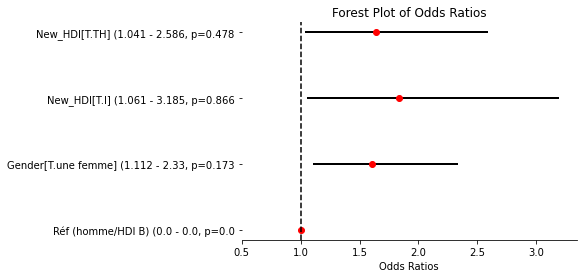
\includegraphics[width=1\textwidth]{../../graph/forestplot_V2_binomiale.png}
	\captionof{figure}{\textbf{Odds-Ratios -  examen $~\sim$ genre et HDI - MOOC V2.}}
\end{figure}

Le risk ratio (RR) représente le risque relatif d'avoir un effet plus ou moins important d'un groupe par rapport à un autre sur un événement. Alors que l'odd-ratio (OR) mesure le rapport de chance d'avoir un effet sur un groupe par rapport à un autre sur un événement. Ces ratios convergent lorsque l'événement se produit rarement.


\subsection{Régression de Poisson}
La Figure 10, donne la forme de la distribution du nombre de vidéos visionnées pour l'ensemble des 3 versions du MOOC.
La figure 11 confirmerait que la distribution n'est pas normale. En effet, en observant l'homoscédasticité des erreurs par 
rapport au modèle théorique, nous nous apercevons que la dispersion (variance) des valeurs observées (en bleu)
n'est pas uniforme autour des valeurs prédites (en rouge). 
Il serait donc inapproprié d'appliquer un modèle de régression linéaire comme la binomiale qui nécessite une distribution normale.
Appliquons maintenant la régression de poisson permettant de comptabiliser statistiquement le nombre de vidéos vues par
genre et par HDI pour ce MOOC. La loi de poisson s'applique sur une distribution non gaussienne mais qui tendrait à l'être, comme celle que l'on observe sur la Figure 8. Nous observons sur cette figure la distribution du nombre de vidéos visionnées pour la version 2 du MOOC.

\begin{figure}[H]
	\centering
	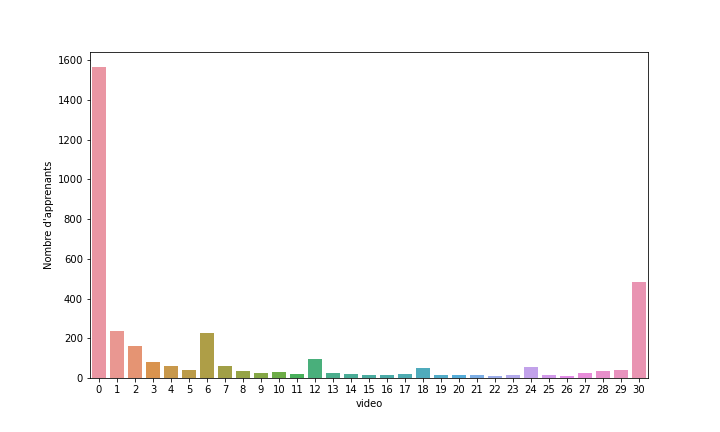
\includegraphics[width=1\textwidth]{../../graph/distribution_poisson.png}
	\caption{\textbf{Distribution du nombre de videos - MOOC V2.}}
\end{figure}

En observant la Figure 9,  nous sommes confiants à 95\% (CI=[1.945, 2.154]) que les apprenants des pays très développés ont significativement (p=0) visionnés bien davantage de vidéos (OR > 2) que les pays pauvres. Elle confirmerait également qu'il n'y a pratiquement aucune différence (OR $\sim 1$) entre les hommes et les femmes sur le nombre de vidéos visionnées.

\begin{figure}[H]
	\centering
	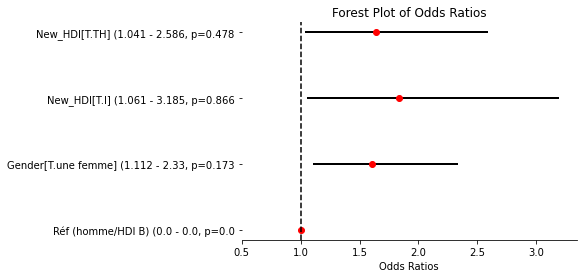
\includegraphics[width=1\textwidth]{../../graph/forestplot_V2_poisson.png}
	\caption{\textbf{odds-ratios du nombre de videos selon le genre et HDI - MOOC V2.}}
\end{figure}

La Figure 10, représente 4 graphiques qui montrent la fiabilité du modèle (graphe 1), la normalité de la distribution du nombre de vidéos (graphe 2), la qualité d'ajustement du modèle (homoscédasticité, graphe 3),    
ainsi que les observations qui auraient un impact sur les prédictions du modèle (graphe 4).
Nous remarquons que la distribution ne tendrait pas vers une distribution normale du nombre de vidéos puisque les valeurs des quantiles observés sont éloignées des valeurs des quantiles du modèle théorique. Le graphe 1 confirmerait que le modèle ne serait pas fiable puisque les résidus des valeurs observées (en bleu) ne sont pas homogènes le long de l'axe horizontale des ordonnées nulles avec des écarts importants par rapport aux valeurs prédites. Le graphe 3, confirmerait la non homoscédasticité, par les grandes variations des résidus, observée sur le graphe 1 avec une mauvaise qualité d'ajustement du modèle. Il est donc impossible de faire des analyses fiables par rapport aux résultats données par la régression de Poisson.



\begin{figure}[H]
	\centering
	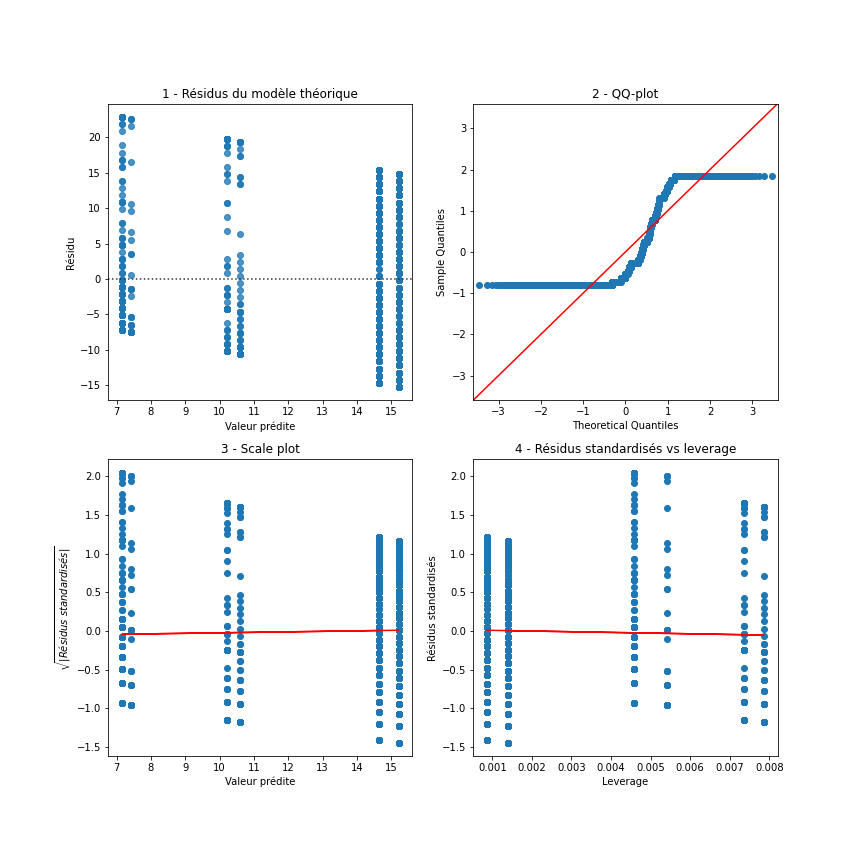
\includegraphics[width=1.2\textwidth]{../../graph/graphs_poisson.png}
	\caption{\textbf{Homoscédasticité - normalité MOOC V2.}}
\end{figure}

\end{document}